%beamer

% Comment/uncomment this line to toggle handout mode
%\newcommand{\handout}{}

%% Beamer-Klasse im korrekten Modus
\ifdefined \handout
\documentclass[handout]{beamer} % Handout mode
\else
\documentclass{beamer}
\fi

%% UTF-8-Encoding
\usepackage[utf8]{inputenc}

\input{../framework/gbi-macros}
\usepackage[blue]{../framework/thwregex}
\usepackage{environ}
\usepackage{bm}
\usepackage{calc}
\usepackage{varwidth}
\usepackage{wasysym}
\usepackage{mathtools}


% Das ist der KIT-Stil
%\usepackage{../TutTexbib/beamerthemekit}
\usepackage[deutsch,titlepage0]{../framework/KIT/beamerthemeKITmod}
\TitleImage[width=\titleimagewd]{../figures/titlepage.jpg}
%\usetheme[deutsch,titlepage0]{KIT}

% Include PDFs
\usepackage{pdfpages}

% Libertine font (Original GBI font)
\usepackage{libertine}
%\renewcommand*\familydefault{\sfdefault}  %% Only if the base font of the document is to be sans serif

% Nicer math symbols
\usepackage{eulervm}
%\usepackage{mathpazo}
\renewcommand\ttdefault{cmtt} % Computer Modern typewriter font, see lecture slides.

\usepackage{csquotes}

%%%%%%

%% Schönere Schriften
\usepackage[TS1,T1]{fontenc}

%% Bibliothek für Graphiken
\usepackage{graphicx}

%% der wird sowieso in jeder Datei gesetzt
\graphicspath{{../figures/}}

%% Anzeigetiefe für Inhaltsverzeichnis: 1 Stufe
\setcounter{tocdepth}{1}

%% Hyperlinks
\usepackage{hyperref}
% I don't know why, but this works and only includes sections and NOT subsections in the pdf-bookmarks.
\hypersetup{bookmarksdepth=subsection} 

%\usepackage{lmodern}
\usepackage{colortbl}
\usepackage[absolute,overlay]{textpos}
\usepackage{listings}
\usepackage{forloop}
%\usepackage{algorithmic} % PseudoCode package 

\usepackage{tikz}
\usetikzlibrary{matrix}
\usetikzlibrary{arrows.meta}
\usetikzlibrary{automata}
\usetikzlibrary{tikzmark}
\usetikzlibrary{positioning}

% Why has no-one come up with this yet? I mean, seriously. -.-
\tikzstyle{loop below right} = [loop, out=-60,in=-30, looseness=7]
\tikzstyle{loop below left} = [loop, out=-150,in=-120, looseness=7]
\tikzstyle{loop above right} = [loop, out=60,in=30, looseness=7]
\tikzstyle{loop above left} = [loop, out=150,in=120, looseness=7]
\tikzstyle{loop right below} = [loop below right]
\tikzstyle{loop left below} = [loop below left]
\tikzstyle{loop right above} = [loop above right]
\tikzstyle{loop left above} = [loop above left]

% Needed for gbi-macros
\usepackage{xspace}

%%%%%%

%% Verbatim
\usepackage{moreverb}

%%%%%%%%%%%%%%%%%%%%%%%%%%%%%%%%%%%% Copy end

%% Tabellen
\usepackage{array}
\usepackage{multicol}
\usepackage{hhline}

%% Bibliotheken für viele mathematische Symbole
\usepackage{amsmath, amsfonts, amssymb}

%% Deutsche Silbentrennung und Beschriftungen
\usepackage[ngerman]{babel}

\usepackage{kbordermatrix}

% kbordermatrix settings
\renewcommand{\kbldelim}{(} % Left delimiter
\renewcommand{\kbrdelim}{)} % Right delimiter

\input{../config.tex}



% define custom \handout command flag if handout mode is toggled  #DirtyAsHellButWell...
\only<beamer:0>{\def\handout{}} %beamer:0 == handout mode

\newcommand{\R}{\mathbb{R}}
\newcommand{\N}{\mathbb{N}}
\newcommand{\Z}{\mathbb{Z}}
\newcommand{\Q}{\mathbb{Q}}
\newcommand{\BB}{\mathbb{B}}
\newcommand{\C}{\mathbb{C}}
\newcommand{\K}{\mathbb{K}}
\newcommand{\G}{\mathbb{G}}
\newcommand{\nullel}{\mathcal{O}}
\newcommand{\einsel}{\mathds{1}}
\newcommand{\Pot}{\mathcal{P}}
\renewcommand{\O}{\text{O}}

\def\word#1{\hbox{\textcolor{blue}{\texttt{#1}}}}
\let\literal\word
\def\mword#1{\hbox{\textcolor{blue}{$\mathtt{#1}$}}}  % math word
\def\sp{\scalebox{1}[.5]{\textvisiblespace}}
\def\wordsp{\word{\sp}}

%\newcommand{\literal}[1]{\textcolor{blue}{\texttt{#1}}}
\newcommand{\realTilde}{\textasciitilde \ }
\newcommand{\setsize}[1]{\ensuremath{\left\lvert #1 \right\rvert}}
\newcommand{\size}[1]{\setsize{#1}}  % Shame on you, TeXStudio...
\newcommand{\set}[1]{\left\{#1\right\}}
\newcommand{\tuple}[1]{\left(#1\right)}
\newcommand{\normalvar}[1]{\text{$#1$}}

% Modified by DJ
\let\oldemptyset\emptyset
\let\emptyset\varnothing % proper emptyset

\newcommand{\boder}{\ensuremath{\mathbin{\textcolor{blue}{\vee}}}\xspace}
\newcommand{\bund}{\ensuremath{\mathbin{\textcolor{blue}{\wedge}}}\xspace}
\newcommand{\bimp}{\ensuremath{\mathrel{\textcolor{blue}{\to}}}\xspace}
\newcommand{\bgdw}{\ensuremath{\mathrel{\textcolor{blue}{\leftrightarrow}}}\xspace}
\newcommand{\bnot}{\ensuremath{\textcolor{blue}{\neg}}\xspace}
\newcommand{\bone}{\ensuremath{\textcolor{blue}{1}}\text{}}
\newcommand{\bzero}{\ensuremath{\textcolor{blue}{0}}\text{}}
\newcommand{\bleftBr}{\ensuremath{\textcolor{blue}{\texttt{(}}}\text{}}
\newcommand{\brightBr}{\ensuremath{\textcolor{blue}{\texttt{)}}}\text{}}

% Fix of \b... commands:

\renewcommand{\boder}{\alor}
\renewcommand{\bund}{\aland}
\renewcommand{\bimp}{\alimpl}
\renewcommand{\bgdw}{\aleqv}
\renewcommand{\bnot}{\alnot}
\renewcommand{\bleftBr}{\alka}
\renewcommand{\brightBr}{\alkz}
\newcommand{\alA}{\word A}
\newcommand{\alB}{\word B}
\newcommand{\alC}{\word C}

\newcommand{\plB}{\plfoo{B}}
\newcommand{\plE}{\plfoo{E}}

\newcommand{\summe}[2]{\sum\limits_{#1}^{#2}}
\newcommand{\limes}[1]{\lim\limits_{#1}}

%\newcommand{\numpp}{\advance \value{weeknum} by -2 \theweeknum \advance \value{weeknum} by 2}
%\newcommand{\nump}{\advance \value{weeknum} by -1 \theweeknum \advance \value{weeknum} by 1}

\newcommand{\mycomment}[1]{}
\newcommand{\Comment}[1]{}

%% DISCLAIMER START 
% It is INSANELY IMPORTANT NOT TO DO THIS OUTSIDE BEAMER CLASS! IN ARTCILE DOCUMENTS, THIS IS VERY LIKELY TO BUG AROUND!
\makeatletter%
\@ifclassloaded{beamer}%
{
	% TODO 
	% no time... later.   (= never -.-)
	% redefine section to ignore multiple \section calls with the same title
}%
{
	\errmessage{ERROR: section command redefinition outside of beamer class document! Please contact the author of this code or read the F-ing disclaimer.}
}%
\makeatother%
%% DISCLAIMER END

\newcounter{abc}
\newenvironment{alist}{
  \begin{list}{(\alph{abc})}{
      \usecounter{abc}\setlength{\leftmargin}{8mm}\setlength{\labelsep}{2mm}
    }
}{\end{list}}


\newcommand{\stdarraystretch}{1.20}
\renewcommand{\arraystretch}{\stdarraystretch}  % for proper row spacing in tables

\newcommand{\morescalingdelimiters}{   % for proper \left( \right) typography
	\delimitershortfall=-1pt  
	\delimiterfactor=1
}

\newcommand{\centered}[1]{\vspace{-\baselineskip}\begin{center}#1\end{center}\vspace{-\baselineskip}}

% for \implitem and \item[bla] stuff to look right:
\setbeamercolor*{itemize item}{fg=black}
\setbeamercolor*{itemize subitem}{fg=black}
\setbeamercolor*{itemize subsubitem}{fg=black}

\setbeamercolor*{description item}{fg=black}
\setbeamercolor*{description subitem}{fg=black}
\setbeamercolor*{description subsubitem}{fg=black}

\renewcommand{\qedsymbol}{\textcolor{black}{\openbox}}

\renewcommand{\mod}{\mathop{\textbf{mod}}}
\renewcommand{\div}{\mathop{\textbf{div}}}

\newcommand{\ceil}[1]{\left\lceil#1\right\rceil}
\newcommand{\floor}[1]{\left\lfloor#1\right\rfloor}
\newcommand{\abs}[1]{\left\lvert #1 \right\rvert}
\newcommand{\Matrix}[1]{\begin{pmatrix} #1 \end{pmatrix}}
\newcommand{\braced}[1]{\left\lbrace #1 \right\rbrace}

% "something" placeholder. Useful for repairing spacing of operator sections, like `\sth = 42`.
\def\sth{\vphantom{.}}

\def\fract#1/#2 {\frac{#1}{#2}} % ! Trailing space is crucial!
\def\dfract#1/#2 {\dfrac{#1}{#2}} % ! Trailing space is crucial!

\newcommand{\Mid}{\;\middle|\;}

\let\after\circ



\def\·{\cdot}
\def\*{\cdot}
\def\?>{\ensuremath{\rightsquigarrow}}  % Fuck you, Latex
\def\~~>{\ensuremath{\rightsquigarrow}}  

\newcommand{\tight}[1]{{\renewcommand{\arraystretch}{0.76} #1}}
\newcommand{\stackedtight}[1]{\renewcommand{\arraystretch}{0.76} \begin{matrix} #1 \end{matrix} }
\newcommand{\stacked}[1]{\begin{matrix} #1 \end{matrix} }
\newcommand{\casesl}[1]{\delimitershortfall=0pt  \left\lbrace\hspace{-.3\baselineskip}\begin{array}{ll} #1 \end{array}\right.}
\newcommand{\casesr}[1]{\delimitershortfall=0pt  \left.\begin{array}{ll} #1 \end{array}\hspace{-.3\baselineskip}\right\rbrace}
\newcommand{\caseslr}[1]{\delimitershortfall=0pt  \left\lbrace\hspace{-.3\baselineskip}\begin{array}{ll} #1 \end{array}\hspace{-.3\baselineskip}\right\rbrace}

\def\q#1uad{\ifnum#1=0\relax\else\quad\q{\the\numexpr#1-1\relax}uad\fi}
% e.g. \q1uad = \quad, \q2uad = \qquad etc.

\newcommand{\qqquad}{\q3uad}
\newcommand{\minusquad}{\hspace{-1em}}

%% Placeholder utils
% \§{#1}   Saves #1 as placeholder and prints it
% \.       Prints an \hphantom with the size of the recalled placeholder.
\def\indentstring{}
\def\§#1{\def\indentstring{#1}#1}
\def\.{{$\hphantom{\text{\indentstring}}$}}
%% Placeholder utils end

\newcommand{\impl}{\ifmmode\ensuremath{\mskip\thinmuskip\Rightarrow\mskip\thinmuskip}\else$\Rightarrow$\fi\xspace}
\newcommand{\Impl}{\ifmmode\implies\else$\Longrightarrow$\fi\xspace}

\newcommand{\derives}{\Rightarrow}

\newcommand{\gdw}{\ifmmode\mskip\thickmuskip\Leftrightarrow\mskip\thickmuskip\else$\Leftrightarrow$\fi\xspace}
\newcommand{\Gdw}{\ifmmode\iff\else$\Longleftrightarrow$\fi\xspace}

% Legacy code from the algo tutorial slides. Perhaps useful. Try with care.
\mycomment{
	\newcommand{\impl}{\ifmmode\ensuremath{\mskip\thinmuskip\Rightarrow\mskip\thinmuskip}\else$\Rightarrow$\xspace\fi}  
	\newcommand{\Impl}{\ifmmode\implies\else$\Longrightarrow$\xspace\fi}
	
	\newcommand{\gdw}{\ifmmode\mskip\thickmuskip\Leftrightarrow\mskip\thickmuskip\else$\Leftrightarrow$\xspace\fi}
	\newcommand{\Gdw}{\ifmmode\iff\else$\Longleftrightarrow$\xspace\fi}
}
	
\newcommand{\gdwdef}{\ifmmode\mskip\thickmuskip:\Leftrightarrow\mskip\thickmuskip\else:$\Leftrightarrow$\xspace\fi}
\newcommand{\Gdwdef}{\ifmmode\mskip\thickmuskip:\Longleftrightarrow\mskip\thickmuskip\else:$\Longleftrightarrow$\xspace\fi}

\newcommand{\symbitemnegoffset}{\hspace{-.5\baselineskip}}
\newcommand{\implitem}{\item[\impl\symbitemnegoffset]}
\newcommand{\Implitem}{\item[\Impl\symbitemnegoffset]}


\newcommand{\forcenewline}{\mbox{}\\}

\newcommand{\bfalert}[1]{\textbf{\alert{#1}}}
\let\elem\in   % I'm a Haskell freak. Don't judge me. :P


\def\|#1|{\text{\normalfont #1}}  % | steht für senkrecht (anstatt kursiv wie sonst im math mode)


% proper math typography
\newcommand{\functionto}{\longrightarrow}
\renewcommand{\geq}{\geqslant}
\renewcommand{\leq}{\leqslant}
\let\oldsubset\subset
\renewcommand{\subset}{\subseteq} % for all idiots out there using subset

\newenvironment{threealign}{%
	\[
	\begin{array}{r@{\ }c@{\ }l}
}{%
	\end{array}	
	\]
}

\newcommand{\concludes}{ \\ \hline  }
\newcommand{\deduction}[1]{
	\begin{varwidth}{.8\linewidth}
		\begin{tabular}{>{$}c<{$}}
			#1
		\end{tabular}
	\end{varwidth}	
}

\definecolor{hoareorange}{rgb}{1,.85,.6}
\newcommand{\hoareassert}[1]{\setlength{\fboxsep}{1pt}\setlength{\fboxrule}{-1.4pt}\fcolorbox{white}{hoareorange}{\ensuremath{\{\;#1\;\}}}\setlength\fboxrule{\defaultfboxrule}\setlength{\fboxsep}{3pt}}

\newcommand{\mailto}[1]{\href{mailto:#1}{{\textcolor{blue}{\underline{#1}}}}}
\newcommand{\urlnamed}[2]{\href{#2}{\textcolor{blue}{\underline{#1}}}}
\renewcommand{\url}[1]{\urlnamed{#1}{#1}}

\newcommand{\hanging}{\hangindent=0.7cm}
\newcommand{\indented}{\hanging}


% \hstretchto prints #2 left-aligned into a box of the width of #1
\def\hstretchto#1#2{%
	\mbox{}\vphantom{#2}\rlap{#2}\hphantom{#1}%
}

\def\vstretchto#1#2{%
	\mbox{}\hphantom{#2}\smash{#2}\vphantom{#1}%
}

% \hstretchtocentered prints #2 centered into a box of the width of #1
\def\hstretchtocentered#1#2{%
	\mbox{}\vphantom{#2}\scalebox{0.5}{\hphantom{#1}}\clap{#2}\scalebox{0.5}{\hphantom{#1}}%
}

% vertical centering
\newcommand{\vertcenter}[1]{%
	\ensuremath{\vcenter{\hbox{#1}}}%
}


%requires \thisyear to be defined (s. config.tex)!
\edef\nextyear{\the\numexpr\thisyear+1\relax}


% --- \frameheight constant ---
\newlength\fullframeheight
\newlength\framewithtitleheight
\setlength\fullframeheight{.92\textheight}
\setlength\framewithtitleheight{.86\textheight}

\newlength\frameheight
\setlength\frameheight{\fullframeheight}

\let\frametitleentry\relax
\let\oldframetitle\frametitle
\def\newframetitle#1{\global\def\frametitleentry{#1}\if\relax\frametitleentry\relax\else\setlength\frameheight{\framewithtitleheight}\fi\oldframetitle{#1}}
\let\frametitle\newframetitle

\def\newframetitleoff{\let\frametitle\oldframetitle}
\def\newframetitleon{\let\frametitle\newframetitle}
% --- \frameheight constant end ---

\newcommand{\fakeframetitle}[1]{%
	\vspace{-2.05\baselineskip}%
	{\Large \textbf{#1}} \\%
	\smallskip
}



\newenvironment{headframe}{\Huge THIS IS AN ERROR. PLEASE CONTACT THE ADMIN OF THIS TEX CODE. (headframe env def failed)}{}
\RenewEnviron{headframe}[1][]{
	\begin{frame}\frametitle{\ }
		\centering
		\Huge\textbf{\textsc{\BODY} \\
		}
		\Large {#1}
		\frametitle{\ }
	\end{frame}
}


\makeatletter
% Provides color if undefined.
\newcommand{\colorprovide}[2]{%
	\@ifundefinedcolor{#1}{\colorlet{#1}{#2}}{}}
\makeatother


\colorprovide{lightred}{red!30}
\colorprovide{lightgreen}{green!40}
\colorprovide{lightyellow}{yellow!50}
\colorprovide{lightblue}{blue!10}
\colorprovide{beamerlightred}{lightred}
\colorprovide{beamerlightgreen}{lightgreen}
\colorprovide{beamerlightyellow}{lightyellow}
\colorprovide{beamerlightblue}{lightblue}
\colorprovide{fullred}{red!60}
\colorprovide{fullgreen}{green}
\definecolor{darkred}{RGB}{115,48,38}
\definecolor{darkgreen}{RGB}{48,115,38}
\definecolor{darkyellow}{RGB}{100,100,0}

\only<handout:0>{\colorlet{adaptinglightred}{beamerlightred}}
\only<handout:0>{\colorlet{adaptinglightgreen}{beamerlightgreen}}
\only<handout:0>{\colorlet{adaptinglightyellow}{beamerlightyellow}}
\only<handout:0>{\colorlet{adaptinglightblue}{beamerlightblue}}
\only<beamer:0>{\colorlet{adaptinglightred}{lightred}}
\only<beamer:0>{\colorlet{adaptinglightgreen}{lightgreen}}
\only<beamer:0>{\colorlet{adaptinglightyellow}{lightyellow}}
\only<beamer:0>{\colorlet{adaptinglightblue}{lightblue}}
\only<handout:0>{\colorlet{adaptingred}{lightred}}
\only<beamer:0>{\colorlet{adaptingred}{fullred}}
\only<handout:0>{\colorlet{adaptinggreen}{lightgreen}}
\only<beamer:0>{\colorlet{adaptinggreen}{fullgreen}}



\newcommand{\TrueQuestion}[1]{
	\TrueQuestionE{#1}{}
}

\newcommand{\YesQuestion}[1]{
	\YesQuestionE{#1}{}
}

\newcommand{\FalseQuestion}[1]{
	\FalseQuestionE{#1}{}
}

\newcommand{\NoQuestion}[1]{
	\NoQuestionE{#1}{}
}

\newcommand{\DependsQuestion}[1]{
	\DependsQuestionE{#1}{}
}

\newcommand{\QuestionVspace}{\vspace{4pt}}
\newcommand{\QuestionParbox}[1]{\begin{varwidth}{.85\linewidth}#1\end{varwidth}}
\newcommand{\ExplanationParbox}[1]{\begin{varwidth}{.97\linewidth}#1\end{varwidth}}
\colorlet{questionlightgray}{gray!23}
\let\defaultfboxrule\fboxrule

% #1: bg color
% #2: fg color short answer
% #3: short answer text
% #4: question
% #5: explanation
\newcommand{\GenericQuestion}[5]{
	\setlength\fboxrule{2pt}
	\only<+|handout:0>{\hspace{-2pt}\fcolorbox{white}{questionlightgray}{\QuestionParbox{#4} \quad\textbf{?}}}
	\visible<+->{\hspace{-2pt}\fcolorbox{white}{#1}{\QuestionParbox{#4} \quad\textbf{\textcolor{#2}{#3}}} \if\relax#5\relax\else\ExplanationParbox{#5}\fi} \\
	\setlength\fboxrule{\defaultfboxrule}
}

% #1: Q text
% #2: Explanation
\newcommand{\TrueQuestionE}[2]{
	\GenericQuestion{adaptinglightgreen}{darkgreen}{Wahr.}{#1}{#2}
}

% #1: Q text
% #2: Explanation
\newcommand{\YesQuestionE}[2]{
	\GenericQuestion{adaptinglightgreen}{darkgreen}{Ja.}{#1}{#2}
}

% #1: Q text
% #2: Explanation
\newcommand{\FalseQuestionE}[2]{
	\GenericQuestion{adaptinglightred}{darkred}{Falsch.}{#1}{#2}
}

% #1: Q text
% #2: Explanation
\newcommand{\NoQuestionE}[2]{
	\GenericQuestion{adaptinglightred}{darkred}{Nein.}{#1}{#2}
}

% #1: Q text
% #2: Explanation
\newcommand{\DependsQuestionE}[2]{
	\GenericQuestion{adaptinglightyellow}{darkyellow}{Je nachdem!}{#1}{#2}
}

% #1: Q text
% #2: Answer
\newcommand{\ContentQuestion}[2]{
	\GenericQuestion{adaptinglightblue}{black}{\minusquad}{#1}{#2}
}

\ifnum\thisyear=2021 \else \errmessage{Old ILIAS link inside preamble. Please update.} \fi

\newcommand{\ILIAS}{\urlnamed{ILIAS}{\myILIASurl}\xspace}
\newcommand{\Klausurtermin}{\myKlausurtermin\xspace}

\newcommand{\Socrative}{\ifdefined\mysocrativeroom \only<handout:0>{socrative.com $\quad \~~> \quad $ Student login \\ Raumname:  \mysocrativeroom\\ \medskip}\else\fi}

\newcommand{\thasse}[1]{
	\ifdefined\ThassesTut #1\xspace \else\fi
}
\newcommand{\daniel}[1]{
	\ifdefined\DanielsTut #1\xspace \else\fi
}
\newcommand{\thassedaniel}[2]{\ifdefined\ThassesTut #1\else\ifdefined\DanielsTut #2\fi\fi\xspace}

\ifdefined\ThassesTut \ifdefined\DanielsTut \errmessage{ERROR: Both ThassesTut and DanielsTut flags are set. This is most likely an error. Please check your config.tex file.} \else \fi \else \ifdefined\DanielsTut \else \errmessage{ERROR: Neither ThassesTut  nor DanielsTut flags are set. This is most likely an error. Please check your config.tex file.} \fi\fi

%\newcommand{\sgn}{\text{sgn}}

%%%%%%%%%%%% INHALT %%%%%%%%%%%%%%%%

%% Wochennummer
\newcounter{weeknum}

%% Titelinformationen
\title[GBI-Tutorium \mytutnumber, Woche \theweeknum]{Grundbegriffe der Informatik \\ Tutorium \mytutnumber}

\subtitle{Woche \theweeknum\xspace |\xspace\mydate{\theweeknum} \\ \myname \ \  \normalfont (\mailto{\mymail})}
\author[\myname]{\myname}
\institute{KIT -- Karlsruher Institut für Technologie}
\date{\mydate{\theweeknum}\ }

% Modified, DJ (better safe than sorry)
\AuthorTitleSep{ – }

%% Titel einfügen
\newcommand{\titleframe}{\frame{\titlepage}}

%% Alles starten mit \starttut{X}
\newcommand{\starttut}[1]{\setcounter{weeknum}{#1}\pdfinfo{
		/Author (\myname)
		/Title  (GBI-Tutorium \mytutnumber, Woche \theweeknum)
	}\titleframe\frame{\frametitle{Inhalt}\tableofcontents} \AtBeginSection[]{%
		\begin{frame}{Wo sind wir gerade?}
		\tableofcontents[currentsection]
	\end{frame}\addtocounter{framenumber}{-1}}}


\newcommand{\framePrevEpisode}{
\begin{headframe}
	\mylasttimestext
\end{headframe}
}

\newcommand{\lastframetitled}[6]{
	\frame{\frametitle{#6}
		\vspace{-#2\baselineskip}
		\begin{figure}[H]
			\centering
			\LARGE \textbf{\textsc{#5}} \\
			\vspace{.2\baselineskip}
			\includegraphics[#1]{#3}
			\vspace{-6pt}
			\begin{center}
				\small \url{#4} 
			\end{center}
		\end{figure} 
	}
}

% #1 number
% #2 title 
% #3 vspace (positive) without unit (\baselineskip)
\newcommand{\xkcdframe}[3]{
	\lastframetitled{width=.96\textwidth}{#3}{xkcd/#1}{http://xkcd.com/#1}{}{#2}
}

\newcommand{\xkcdframevert}[3]
{
	\lastframetitled{height=.96\frameheight}{#3}{xkcd/#1}{http://xkcd.com/#1}{}{#2}
}

% #1 number
% #2 title 
% #3 vspace (positive) without unit (\baselineskip)
% #4 \includegraphics[] optional parameters
\newcommand{\xkcdframecustom}[4]
{
	\lastframetitled{#4}{#3}{xkcd/#1}{http://xkcd.com/#1}{}{#2}
}

\newcommand{\slideThanks}{
	\begin{frame}
	\frametitle{Credits}
	\begin{block}{}
		An der Erstellung des Foliensatzes haben mitgewirkt:\\[1em]
		Daniel Jungkind \\
		Thassilo Helmold \\
		Philipp Basler \\
		Nils Braun \\
		Dominik Doerner \\
		Ou Yue \\
		Max Schweikart
	\end{block}
\end{frame}
}

%% Wörter DEPRECATED! DO NOT USE
\newcommand{\code}[1]{$\mathbf{#1}$}

\morescalingdelimiters

\begin{document}
\starttut{3}

\section{Organisatorisches}

\begin{frame}{Zu Übungsblatt \#1}
	Schnitt: \quad 15,8 / 20~P

	\begin{itemize}[<+->]
		\item 20 von 24 TutandInnen haben etwas abgegeben. Sehr schön!
		\item Die Musterlösung findet ihr im \ILIAS unter Übungsblätter
		\item Korrekturen gibt es jetzt!
		\item Ich habe ein Übungsblatt erst diese Woche erhalten, die Punktevergabe muss ich dazu noch abklären
	\end{itemize}
\end{frame}

\begin{frame}{Zu Übungsblatt \#1}	
	\begin{itemize}[<+->]
		\item Erstmal: Volle Punktzahl ist utopisch. Fehler macht man, um daraus zu lernen – dazu sind ÜBs da
		\item Für falsche Notationen habe ich beim ersten Blatt teilweise noch nichts abgezogen - in Zukunft gibt es für falsche Notation Abzüge!
	\end{itemize}
\end{frame}

\begin{frame}{Zu Übungsblatt \#1}
	Die häufigsten Fehler:
	\begin{itemize}[<+->]
		\item Wenn in der Aufgabenstellung steht: \textit{Geben Sie ein $x$ an sodass gilt: ...}, dann genügt es ein solches $x$ anzugeben
		\implitem Keine Begründung gefordert!
		\implitem Für eine falsche Begründung gibt es Abzüge, auch wenn keine gefordert
		\item \textbf{All-Aussagen}, also Aussagen mit \textit{Für alle $x$ mit ... gilt ...} könnt ihr mit \textbf{einem Gegenbeispiel} widerlegen.
		\item ...aber ihr könnt sie \textbf{nicht} mit nur einem Beispiel beweisen. Ein Beweis für eine All-Aussage muss für alle solche Elemente gelten!
		\item \textbf{Existenz-Aussagen}, also Aussagen mit \textit{Es existiert ein $x$ sodass ... gilt} könnt ihr mit einem Beispiel beweisen.
		\item ...aber wenn ihr sie widerlegen wollt, müsst ihr das für alle möglichen $x$ tun.
	\end{itemize}
\end{frame}

\begin{frame}{Zu Übungsblatt \#1}
	Die häufigsten Fehler:
	\begin{itemize}[<+->]
		\item Gebt nur eine Lösung an. Wenn ihr mehrere angebt und eine davon falsch ist, muss ich die falsche werten.
		\implitem Gebt nur so viel an wie gefordert ist, ihr könnt dafür nur Abzug bekommen!
		\item Wenn in der Aufgabenstellung steht dass eine Aussage wahr bzw. falsch ist, dann ist sie das auch.
		\item Definiert alle Variablen, die ihr benutzt! \\
			z.B. in Aufgabe 1.3c): \textit{Es sei $a\in (A \cap B)\cup C$}
		\item Sätze aus der Vorlesung müsst ihr nicht abschreiben, der Name reicht, z.B. $ a + b \stackrel{kommutativ}{=} b + a$
	\end{itemize}
\end{frame}

\begin{frame}{Zu Übungsblatt \#1}
	Die häufigsten Fehler:
	\begin{itemize}[<+->]
		\item Unterscheidet Mengen und Aussagen! \\
		Passt mit euren \textbf{Operatoren} auf: Für Mengen $A,B$ sind $A \Rightarrow B$, $A \Leftarrow B$ und $A \Leftrightarrow B$ nicht definiert.
		\implitem Ihr könnt euch mit $x \in A \Rightarrow x \in B$, $A \subseteq B$, ... Abhilfe schaffen.
		\implitem Wenn es um Mengengleichheit geht, könnt ihr einfach $=$ benutzen \\
			z.B. Aufgabe 1.1c): $(B \backslash (B \cup A)) \cup ((A \cup B) \backslash ((A \backslash B) \cup (B \backslash A))) = (B \backslash A) \cup (A \cap B)$
		\item Für eine Menge $A$ haben wir $\bar{A}$ / $\neg A$ / $A^C$ / das ``allgemeine'' Komplement nicht definiert.
		\implitem Stattdessen $x \not\in A$ benutzen
		\item Unterscheidet $\in$ und $\subseteq$! \\
			Insbesondere ist $A$ mit $A \subseteq 2^{\mathbb{N}_0}$ eine Menge von Mengen von natürlichen Zahlen und $B$ mit $B \in 2^{\mathbb{N}_0}$ eine Menge von natürlichen Zahlen.
	\end{itemize}
\end{frame}

\begin{frame}{Zu Übungsblatt \#1}
	Zu guter Letzt:
	\begin{itemize}[<+->]
		\item Bearbeitet die Aufgaben selbstständig oder mit eurem Abgabepartner
		\item Am Besten klappt es mit einem Partner, was auch die Punkteverteilung zeigt
		\item Bleibt dabei! Übung macht den Meister
	\end{itemize}
\end{frame}


\section{Was beim letzten Mal geschah...}

\framePrevEpisode

\begin{frame}{Kahoot!}
	\begin{itemize}[<+->]
		\item Kahoot! ist ein anonymes Online-Quiz
		\item Ihr bekommt Punkte für schnelles und richtiges raten
		\item Ich schalte das Quiz frei und ihr könnt über \url{https://kahoot.it} beitreten
		\item Das Kahoot! könnt ihr euch später nochmal unter diesem Link angucken: \\
			\url{https://create.kahoot.it/share/gbi-woche-3/b3d43857-eb88-4897-b04a-6dca27b46518}
	\end{itemize}
\end{frame}


%\subsection{Wahr oder Falsch?}
%\begin{frame}[t]{Wahr oder Falsch?}
%	\FalseQuestionE{Eine Funktion muss linkseindeutig sein.}{\impl Eine Funktion muss rechtseindeutig \textbf{und linkstotal} sein.}
%	\TrueQuestion{Eine injektive Funktion ist linkseindeutig.}
%	\TrueQuestion{Eine surjektive Funktion ist rechtstotal.}
%	\FalseQuestion{Jede Relation ist eine Funktion.}
%	\TrueQuestion{Jede Funktion ist eine Relation.}
%\end{frame}

%\begin{frame}[t]{Wahr oder Falsch?}
%	\delimitershortfall=0pt
%	\FalseQuestionE{$\word{aaba} \in \{ \word a, \word b\}^2\times\{\word a,\word b\}^2$}{Aber: $(\word{aa}, \word{ba}) \in \{\word a, \word b\}^2\times\{\word a, \word b\}^2$}
%	\FalseQuestionE{$\setsize{\{ \eps \}} = 0$}{$\{ \eps \} \neq \{\}$}
%	\FalseQuestionE{Wenn $\eps \in A^*$, dann $\size{\eps^3} = 3$.}{$\size{\eps^3} = 0$; außerdem gilt $\eps \in A^*$  immer, also für alle Alphabete $A$.}
%\end{frame}

\section{Binäre Operatoren}
\begin{frame}
	\begin{block}{Binäre Operatoren}
		Eine binäre Operation auf einer Menge $M$ ist eine Abbildung:
		\[ \diamond: M \times M \to M \]
		Üblicherweise benutzt man (wie bei manchen Relationen) die Infixschreibweise, z.B. $m_1 \diamond m_2$ statt  $\diamond(m_1,m_2)$.
	\end{block} \pause
	\begin{block}{Eigenschaften}
		Die Operation $\diamond$ heißt kommutativ, wenn gilt:
		\[ \forall x \in M \ \forall y \in M: x \diamond y = y \diamond x \]
		
		Die Operation $\diamond$ heißt assoziativ, wenn gilt:
		\[ \forall x \in M \ \forall y \in M \ \forall z \in M : (x \diamond y) \diamond z = x \diamond (y \diamond z) \]
	\end{block} \pause
\end{frame}

\section{Induktive Definitionen}

\begin{frame}{Zum Aufwärmen: Domino}
	Drei Dominosteine sind mit gleichem Abstand (kleiner halbe Größe) in einer Reihe aufgestellt. Wir stoßen den ersten Stein der Reihe in Richtung des zweiten Steins um. \\
	Wird der dritte Stein umfallen? Kann man das (einfach) beweisen? \\[1em]
	\pause
	Nun stehen (abzählbar) unendlich viele Dominosteine wie oben hintereinander. Wieder stoßen wir den ersten Stein um. \\
	Wird jeder Stein irgendwann umfallen? Kann man das (einfach) beweisen? \\[1em]
	\pause
	Werden irgendwann alle Steine umgefallen sein? \\
	\pause Nein, denn für jeden Zeitpunkt können wir (mindestens) einen Stein angeben, der noch nicht umgefallen ist.\\
	Wir sehen also: Alle Steine fallen um, aber es sind niemals alle umgefallen.
\end{frame}

\newcommand{\Fib}{\mathcal{F}\hspace{-1pt}}

\begin{frame}{Induktive Definitionen}
	\begin{exampleblock}{Beispiel: \emph{Fibonacci}-Reihe}
		\begin{align*}
		\Fib_0 &:= 0 \\
		\Fib_1 &:= 1 \\
		\text{Für } n \geq 0: \quad \Fib_{n+2} &:= \Fib_{n+1} + \Fib_n 		
		\end{align*}
		\pause
		\begin{table}
			\centering
			\begin{tabular}{|c|c|c|c|c|c|c|c|c|c|c|}
				\hline
				$n$ & 0 & 1 & 2 & 3 & 4 & 5 & 6 & 7 & 8 & 9 \\ \hline
				$\Fib_n$ & 0 & 1 & 1 & 2 & 3 & 5 & 8 & 13 & 21 & 34 \\ \hline
			\end{tabular}
		\end{table}
		
		\pause
		\textbf{Wohldefiniertheit}: 
		\begin{itemize}
			\item Für alle Fälle etwas definieren 
			\item Nicht für einen Fall was Widersprüchliches definieren
		\end{itemize}
		
	\end{exampleblock}
	
\end{frame}

%\section{Vollständige Induktion}

\morescalingdelimiters

% Induktion Vorstellung
\begin{frame}{Vollständige Induktion}
	Wir haben: Aussage $A_n$ für alle $n \in \N_0$ \quad (z.B. $A_n$: „$\size{\word{a}^n} = n$“) \\
	Wir wollen beweisen: $A_n$ ist für alle $n \in \N_0$ wahr \\[0.5em]
	\pause
	Zeige dazu: \centered{	
		$A_n$ ist für $n = 0$ wahr  \\
		\textbf{und} \\
		Wenn $A_n$ für ein $n \in \mathbb{N}_0$ wahr ist, dann ist auch $A_{n+1}$ wahr 
	}
\end{frame}

\begin{frame}[t]{Vorgehen}
	\only<1-3|handout:1>{
		Behauptung: \quad $\forall n \in \N_0: (n^3 - n) \text{ ist durch 3 teilbar (tb)}$.
		\pause
		\begin{block}{Induktionsanfang (IA)}
			Beweise die Aussage für die erste Zahl (Basisfall):\\
			$n = 0 \impl (0^3 - 0) = 0$ ist durch 3 tb. \; \textbf{\checked}
		\end{block}
		\pause
		\bigskip
	}
	\only<3-|handout:1-2>{
		Wir nehmen ein $n$, von dem wir schon gezeigt haben, dass die Aussage gilt:\\ 
		\vspace{-.5\baselineskip}
		\begin{block}{Induktionsvoraussetzung (IV)}
			Für \textbf{ein beliebiges (aber festes)} $n \in \N_0$ gelte: $(n^3 - n)$ ist durch 3 tb. 
		\end{block}
	}
	\pause
	\only<4-|handout:2>{
		\begin{block}{Induktionsschritt (IS)}
			Zeige die Aussage für $n+1$, verwende dabei die IV (und \textbf{dasselbe} $n$ wie in der IV!).\\
			\pause
			\medskip
			Wir formen erst mal um:
			\begin{align*}
			(n+1)^3 - (n+1) &= n^3 + 3n^2 + 3n + 1 - n - 1 \\
			&= (n^3 - n) + (3n^2 + 3n) \\
			&= \underbrace{(n^3-n)}_{\shortstack{\footnotesize nach IV \\ \footnotesize durch 3 tb.}} + \underbrace{3 \* (n^2 + n)}_{\shortstack{\footnotesize offensichtlich \\ \footnotesize durch 3 tb.}}. \qed
			\end{align*}
		\end{block}
	}
	
\end{frame}

\begin{frame}{Induktionsvoraussetzung}
	\Huge \centering
	\alert{
		„Für \textbf{ein} $n \in \N_0$ gelte ...“ \\
		\bigskip
		{ \LARGE
		Nicht: „Für alle...“,\\
		das wollen wir mit der Induktion ja erst zeigen!
		}
	}
\end{frame}

\begin{frame}[t]{Vollständige Induktion}
	\begin{itemize}
		\item Der Schraubenzieher im Beweis-Werkzeugkasten des Informatikers
		\item \textbf{Einfaches} Prinzip (Muss man \textit{verstehen}, reines Auswendiglernen des Schemas kann schief gehen!), vielfältige Anwendungsmöglichkeiten
		\item \textbf{Variationen} möglich: Induktionsanfang bei $1, 42, ...$
	\end{itemize}
	
	\FalseQuestionE{Ich benutze für jeden Beweis Induktion.}{Mit einem Schraubenzieher bekommt man keinen Nagel in die Wand.}
\end{frame}


\begin{frame}{Zum Aufwärmen: Vogelfarben}
	Wir zeigen nun:\\[2em]
	{\LARGE
	Alle Vögel haben die gleiche Farbe!}\\
	\bigskip
	\only<beamer:0>{Achtung: Dieser Beweis ist natürlich \textbf{kaputt}!}
\end{frame}

\begin{frame}[t]{Zum Aufwärmen: Vogelfarben}
	\only<1|handout:1>{
		Das machen wir mit \textbf{vollständiger Induktion} und zeigen die folgende, äquivalente Aussage: \\
	}
	
	\only<1-3|handout:1-2>{
		\[
			\begin{array}{r@{\ }l}
			\forall n \in \N_+ : &\text{ In jeder Menge, die genau } n \text{ Vögel enthält,} \\
								 &\text{ haben alle Vögel die gleiche Farbe.}
			\end{array}
		\]
		
	}
	
	\only<2-3|handout:2>{	
		\begin{block}{Induktionsanfang}
			$n = 1$: Wenn eine Menge genau einen Vogel enthält, dann haben
			offensichtlich alle Vögel die gleiche Farbe. \textbf{\checked}
		\end{block}
	}
	\only<3|handout:2>{
		\begin{block}{Induktionsvoraussetzung}
			Für ein beliebiges aber festes $n$ gelte: In jeder
			Menge, die genau $n$ Vögel enthält, haben alle Vögel die gleiche Farbe.
		\end{block}
	}

	\only<4-5|handout:3-4> {
	\begin{block}{Induktionsschritt}
		\only<4|handout:3>{
			Wir zeigen die Aussage für $n+1$: Sei also $M$ eine Menge,
			die genau $n+1$ Vögel enthalte. Wir stellen uns vor, dass die Vögel
			alle nebeneinander sitzen:
		}
	
		\begin{figure}
			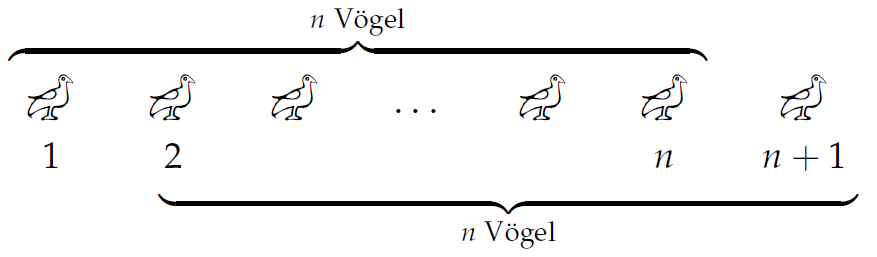
\includegraphics[scale=0.4]{induktion_voegel}
			\centering
		\end{figure}
	
		\only<5|handout:4>{
			Die Vögel $1, 2, ..., n$ bilden eine Menge mit genau $n$ Vögeln. Also haben sie nach IV alle die gleiche Farbe.\\ 
			Die Vögel $2, 3, ..., n + 1$ bilden auch eine Menge mit genau $n$ Vögeln. Also haben nach IV auch diese alle die gleiche Farbe.\\
			Damit haben auch die Vögel $1$ und $n + 1$ die gleiche Farbe, also haben alle Vögel die gleiche Farbe. $\qed$
		}
	\end{block}
	}
\end{frame}

\begin{frame}[t]{Vogelfarben: Auflösung}
	\begin{block}{Was geht schief?}
		\begin{figure}
			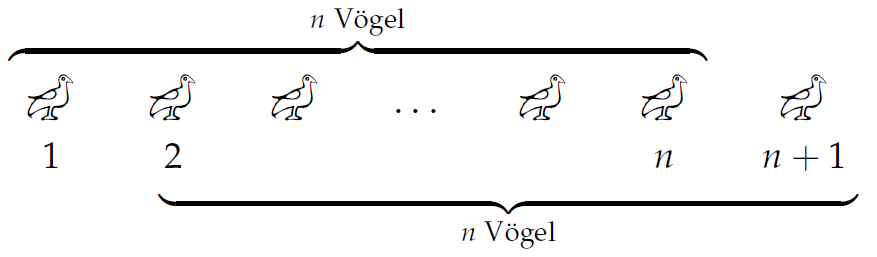
\includegraphics[scale=0.4]{induktion_voegel}
			\centering
		\end{figure}
		\pause
		Hübsches Bild. Scheint sauber. Ist bloß für $n=2$ völlig kaputt, die beiden Teilmengen \textbf{überlappen sich} dann nämlich \textbf{nicht}. \\
		\impl Wir können nicht sagen, dass der erste und letzte Vogel immer die gleiche Farbe haben. (Und wenn schon zwei Vögel nicht immer die gleiche Farbe haben, dann drei etc. auch nicht.) \\
		\impl Ganze Induktion \textbf{kaputt}. \frownie
	\end{block}	
	%Das Bild ist zwar außerordentlich hübsch, suggeriert aber leider etwas, was nicht immer stimmt: Für $n = 2$ überlappen sich die Teilmengen „ohne den ersten“ und „ohne den letzten“ Vogel nicht. Es ist also nicht erzwungen, dass beide Vögel die gleiche Farbe haben. (Und das macht „alles weitere“ auch kaputt: Wenn nicht immer 2 Vögel die gleiche Farbe haben, dann auch nicht immer 3 Vögel, usw.)
\end{frame}

% Induktion Übung

\begin{frame}{Und jetzt ihr}
	Behauptung: \[\forall n \in \N_+ : \sum_{k=0}^{n}{\frac{1}{2^k}} = 2 \* \tuple{1 - \frac{1}{2^{n+1}}}\]
	\pause
	\begin{block}{Induktionsanfang}
		$n = 1$: $\sum_{k=0}^{1}{\frac{1}{2^k}} = \frac{3}{2} = 2 \* \frac{3}{4}$. \; \textbf{\checked}
	\end{block}
	\pause
	\begin{block}{Induktionsvoraussetzung}
		Für ein $n \in \N_0$ gelte: $\sum_{k=0}^{n}{\frac{1}{2^k}} = 2 \* \tuple{1 - \frac{1}{2^{n+1}}}$.
	\end{block}
\end{frame}

\begin{frame}{Und jetzt ihr}
	\uncover<+->{}
	\begin{block}{Induktionsschritt}
		Zeige die Aussage für $n+1$:\\
		\begin{align*}
			\sum_{k=0}^{n+1}{\frac{1}{2^k}}
				&= \uncover<+->{\underbrace{\sum_{k=0}^{n}{\frac{1}{2^k}}}_{\stackrel{\text{IV}}{=} 2 \* \tuple{1 - \frac{1}{2^{n+1}}}} + \frac{1}{2^{n+1}}}\\
				\uncover<+->{&= 2 \* \left(1 - \frac{1}{2^{n+1}}\right) + \frac{1}{2^{n+1}}\\
				&= 2 \* \left(1 - \frac{2}{2^{n+2}} + \frac{1}{2^{n+2}}\right)\\
				&= 2 \* \left(1 - \frac{1}{2^{(n+1)+1}}\right). \qed}
		\end{align*}
	\end{block}
\end{frame}

% Induktion Wörter Länge
\begin{frame}{Und jetzt mit Wörtern}
	\begin{block}{Behauptung}
		Seien $A, B$ zwei beliebige Alphabete. Definiere die Funktion $f \from A^* \functionto A^*$,
		\begin{align*}
			f(\eps) &:= \eps \\
			\text{Für } w \in A^*, \mu \in A: \quad f(\mu \* w) &:= 
			\begin{cases}
				\mu \* f(w), &\mu \in B \\
				f(w), &\text{sonst}
			\end{cases}\\
		\end{align*}
	
	Dann gilt $\forall w \in A^*: \size{f(w)} \le \size w$.
	\end{block}
\end{frame}

\begin{frame}{Und jetzt mit Wörtern}
	Induktion über die Wortlänge ($n = \size w$):\\[0.5em]
	\pause
	\begin{block}{Induktionsanfang}
		$n = 0$: Nur das leere Wort hat Länge 0. Also $w = \eps$.\\
		$f(\eps) = \eps \impl \size{f(w)} = \size w = 0$. \; \textbf{\checked}
	\end{block}
	\pause
	\begin{block}{Induktionsvoraussetzung}
		Für \textbf{ein} $n \in \N_0$ gelte: Für alle Wörter der Länge $n$ über $A$ (also $w \in A^n$) ist $\size{f(w)} \le \size w$.
	\end{block}
\end{frame}

\begin{frame}{Und jetzt mit Wörtern}
	\begin{block}{Induktionsschritt}
		Zeige die Aussage für $n+1$:\\
		Sei $w \in A^{n+1}$ ein Wort der Länge $n+1$.\\
		\pause
		Dann teilen wir es auf in $w = \mu \* v$, wobei $\mu \in A$ und $v \in A^n$.\\
		Nach IV gilt: $\size{f(v)} \le \size v$.\\
		\pause
		\smallskip
		\textbf{Fall 1}: \\
			\quad $\mu \in B$: $f(w) = \mu \* f(v)$ \\
			\quad \impl $\size{f(w)} = 1 + \size{f(v)} \le 1 + \size v = 1+n = \size w$.\\
		\pause
		\smallskip
		\textbf{Fall 2}: \\
			\quad $\mu \notin B$: $f(w) = f(v)$ \\
			\quad \impl $\size{f(w)} = \size{f(v)} \le \size v = n \le n+1 = \size w$.\\
		\pause
		\smallskip
		Also gilt: $\size{f(w)} \le \size w. \qed$
	\end{block}
\end{frame}

\section{Aussagenlogik}

%\thasse{ % No time this year...
%	\frame{
%		\frametitle{Ein bekanntes Logikrätsel}
%		\vspace{-2pt}
%		\begin{figure}[H]
%			\centering
%			\only<1|handout:1>{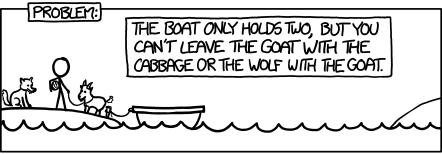
\includegraphics[scale=1]{xkcd/logic_boat_problem}}
%			\only<2|handout:2>{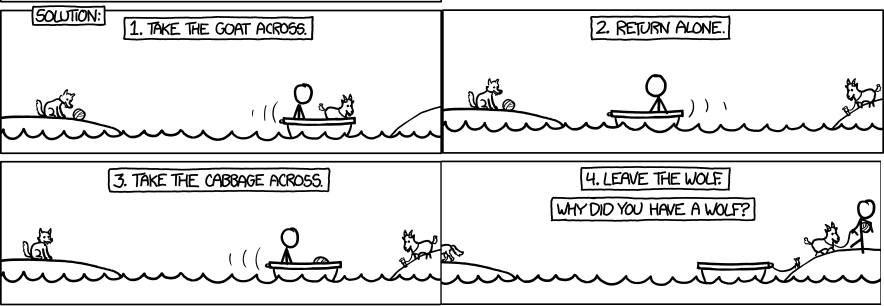
\includegraphics[scale=0.35]{xkcd/logic_boat_sol}}
%			\vspace{-2pt}
%			\url{http://xkcd.com/1134/}
%		\end{figure} 
%	}
%}

\begin{frame}{Aussagenlogik}
	Aussagen sind Sätze, die entweder \textbf{wahr} oder \textbf{falsch} sind.\\
	Deren Wahrheitswert muss dabei nicht unbedingt bekannt oder \enquote{tatsächlich ermittelbar} sein.
	
	\pause
	\begin{Beispiel}
		\begin{itemize}
			\item „$ 1 + 1 = 2 $“ ist eine Aussage. Sie ist wahr.
			\item \enquote{Es gibt nur endlich viele Primzahlen.} ist eine Aussage. Sie ist falsch.
			\pause
			\item Die Goldbachsche Vermutung (Jede gerade Zahl größer 2 ist Summe zweier Primzahlen) \pause ist eine Aussage. Ihr Wahrheitswert ist unbekannt.
			\pause
			\item „Die Welt wird am 11.11.11111 untergehen.“ \pause ist auch eine Aussage. Wir werden ihren Wahrheitswert aber wohl niemals ermitteln können.
			\pause
			\item \enquote{Gelb} ist keine Aussage.
			\pause
			\item \enquote{Dieser Satz ist falsch.} \pause ist keine Aussage. Dem Satz kann offensichtlich kein Wahrheitswert zugeordnet werden.
		\end{itemize}
	\end{Beispiel}
\end{frame}

\begin{frame}{Zwei Grundsätze der Aussagenlogik}
	
	\begin{itemize}
		\pause
		\item[1.] Jede Aussage ist \textbf{entweder} wahr \textbf{oder} falsch.\\
		Wir schreiben im Folgenden $\BB= \{\W, \F\}$
		\pause
		\item[2.] Der Wahrheitswert einer \textbf{zusammengesetzten} Aussage ist durch die
		Wahrheitswerte der \textbf{Teilaussagen} eindeutig festgelegt. \\
		\enquote{$2 + 2 = 5 \; \bimp \; \text{Pinguine können fliegen}$} ist \textbf{wahr}.\\[0.2em]
		%TODO
		%Ex falso quodlibet
	\end{itemize}

	\impl Weg vom Inhalt und betrachte stattdessen \textbf{Aussagevariablen}.
\end{frame}

\begin{frame}{Syntax}
	\begin{Definition}
		$Var_{AL}$ ist die Menge aller \textbf{Aussagevariablen}. \\
		Wir bilden aussagenlogische Formeln als Wörter über dem Alphabet $A_{AL} = \{ \bleftBr, \brightBr, \bnot, \bund, \boder, \bimp \} \cup Var_{AL}$ 
	\end{Definition}
	\pause
	\begin{Definition}
		$For_{AL}$ ist die Menge aller \textbf{syntaktisch korrekten Formeln} über $Var_{AL}$.\\
		\medskip
		(VL: induktive Definition über Konstruktionsabbildungen) \\
		Klammern, die überflüssig sind, können weg. Wir lesen es dann wie gewohnt (\enquote{$\bnot$} vor \enquote{ $\bund$} vor \enquote{ $\boder$} vor \enquote{ $\bimp$}  {\small \#PunktVorStrichUndSo}).
	\end{Definition}
	\pause
	\begin{Beispiel}
		$$Var_{AL} = \{\alA, \alB, \alC\}$$
		$$For_{AL} = \set{\alka \alA  \bimp \alB \alkz \boder \bnot \alB \bund \alC, \ \alC \bimp \alka \bnot \alC \alkz, ...}$$ 
	\end{Beispiel}
\end{frame}

\begin{frame}{Semantik}
	Die Semantik einer aussagenlogischen Formel wird durch ihre \textbf{Auswertung} bestimmt.\\
	Hierbei werden den Operatorsymbolen aus $A_{AL}$ boolesche Funktionen zugeordnet.
	
	\pause
	\begin{Definition}
		Eine \textbf{boolesche Funktion} ist eine Abbildung der Form
		$f \from \BB^n \functionto \BB$.
	\end{Definition}

	\pause
	\begin{Beispiel}
		\enquote{Handelsübliche} boolesche Funktionen sind  $b_{\bnot}$,
		$b_{\bund}$, $b_{\boder}$ und $b_{\bimp}$. 
	\end{Beispiel}
\end{frame}

\begin{frame}{Semantik}
	\let\w\W
	\let\f\F
	\begin{center}
		\begin{huge}
			$$\only<1-2|handout:1>{\bnot}\only<3-4|handout:2>{\bund}\only<5-6|handout:3>{\boder}\only<7-8|handout:4>{\bimp}$$
		\end{huge}
		Wahrheitstabelle: \\
		\medskip
		\only<1-2|handout:1>{
			\begin{tabular}{|c|c|}
				\hline 
				$A$ &  $\bnot A$ \\
				\hline
				\w & \uncover<2|handout:1>{\f} \\
				\hline
				\f & \uncover<2|handout:1>{\w} \\
				\hline
			\end{tabular}
		}
		\only<3-4|handout:2>{ 
			\begin{tabular}{|c|c|c|}
				\hline 
				$A$ & $B$ & $A \mathop{\bund} B$ \\
				\hline
				\w & \w & \uncover<4|handout:2>{\w} \\
				\hline
				\w & \f & \uncover<4|handout:2>{\f} \\
				\hline
				\f & \w & \uncover<4|handout:2>{\f} \\
				\hline
				\f & \f & \uncover<4|handout:2>{\f} \\
				\hline
			\end{tabular}
		}
		\only<5-6|handout:3>{ 
			\begin{tabular}{|c|c|c|}
				\hline 
				$A$ & $B$ & $A \mathop{\boder} B$ \\
				\hline
				\w & \w & \uncover<6|handout:3>{\w} \\
				\hline
				\w & \f & \uncover<6|handout:3>{\w} \\
				\hline
				\f & \w & \uncover<6|handout:3>{\w} \\
				\hline
				\f & \f & \uncover<6|handout:3>{\f} \\
				\hline
			\end{tabular}
		}
		\only<7-8|handout:4>{
			\begin{tabular}{|c|c|c|}
				\hline 
				$A$ & $B$ & $A \mathop{\bimp} B$ \\
				\hline
				\w & \w & \uncover<8|handout:4>{\w} \\
				\hline
				\w & \f & \uncover<8|handout:4>{\f} \\
				\hline
				\f & \w & \uncover<8|handout:4>{\w} \\
				\hline
				\f & \f & \uncover<8|handout:4>{\w} \\
				\hline
			\end{tabular}
		}
	\end{center}
\end{frame}

\begin{frame}{Semantik}
	Wenn wir den Wahrheitswert einer \textbf{zusammengesetzten} Aussage bestimmen wollen, brauchen wir die Werte der \textbf{verwendeten Aussagenvariablen}. \\
	\begin{Definition}
		Sei $V \subseteq Var_{AL}$ die Menge der verwendeten Aussagevariablen.\\
		Eine Funktion $I \from V \functionto \BB$ bezeichnet man als \textbf{Interpretation}.
	\end{Definition}
	
	

\end{frame}

\begin{frame}{Auswertung}
	\begin{Definition}
		Sei $I$ eine Interpretation. Dann liefert die Abbildung $val_I(A)$ den Wahrheitswert zu einer aussagenlogischen Formel $A$. \\
		\medskip
		Diese Funktion nennen wir \textbf{Auswertung} und berechnen sie schrittweise, z.~B.:
	\end{Definition}
	
	\begin{align*}
	&val_I(\alka\alA \bimp \alB\alkz \boder \bnot \alB)  \\
	\visible<2->{= \;&b_{\boder} (val_I(\alA\bimp \alB), val_I(\bnot \alB)) \\}
	\visible<3->{= \;&b_{\boder} (b_{\bimp} (val_I(\alA), val_I(\alB)), b_{\bnot}(val_I(\alB))) \\}
	\visible<4->{= \;&b_{\boder} (b_{\bimp} (I(\alA), I(\alB)), b_{\bnot}(I(\alB))) \\}
	\end{align*}
\end{frame}

\begin{frame}{Auswertung}
	\begin{Definition}
		Eine \textbf{Tautologie} ist eine aussagenlogische Formel, bei der für alle möglichen Interpretationen $I$ gilt: $val_I(A) = \W$. \\
		\impl Schreibweise: \quad $\models A$ \\
		\medskip
		
		\pause
		Zwei aussagenlogische Formeln $A$ und $B$ heißen \textbf{äquivalent}, wenn für jede beliebige Interpretation $I$
		$$val_I(A) = val_I(B)$$
		gilt. \\
		\impl Schreibweise: \quad $A \equiv B$
	\end{Definition}
\end{frame}

% TODO
%\begin{frame}[t]{Auswertung}
%	\only<all:1>{
\includegraphics[scale=0.65]{al_uebung_1}\\[2em]
%	Quelle: GBI-Übung 2015/2016}
%	\only<all:2>{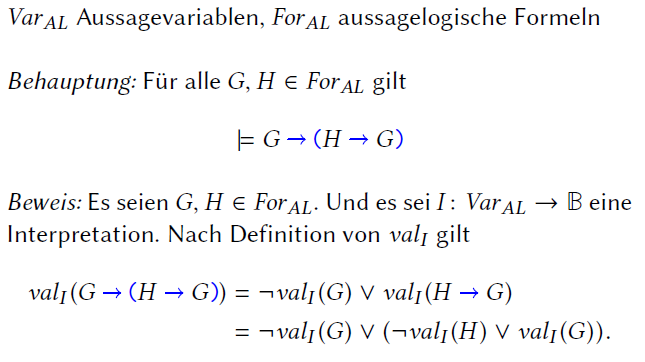
\includegraphics[scale=0.65]{al_uebung_2}}
%	\only<all:3>{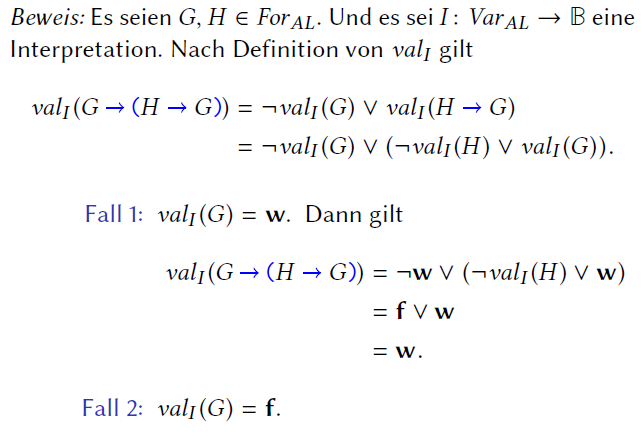
\includegraphics[scale=0.65]{al_uebung_3}}
%	\only<all:4>{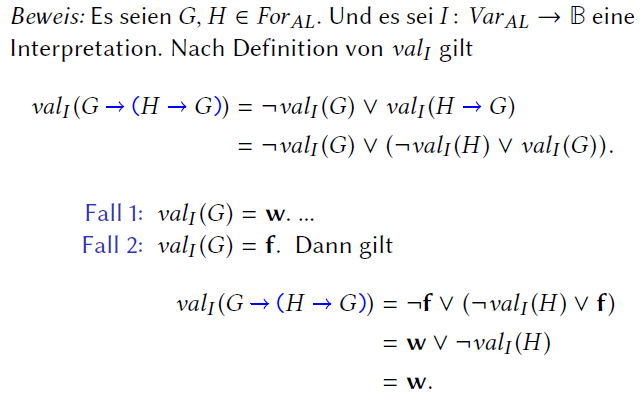
\includegraphics[scale=0.65]{al_uebung_4}}
%	\only<all:5>{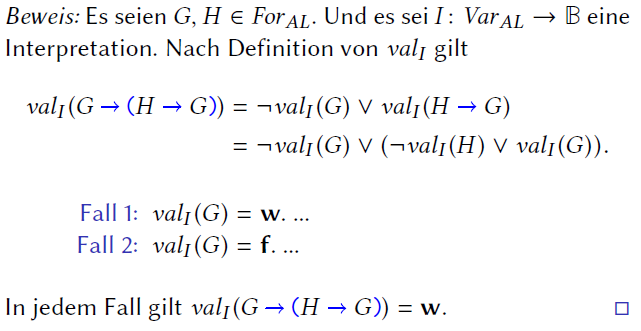
\includegraphics[scale=0.65]{al_uebung_5}}
%\end{frame}

\begin{frame}{Semantik}
	
	Möchte man eine AL-Formel für alle möglichen Interpretationen auswerten, so macht man dies meist in Form einer \textbf{Wahrheitstabelle}.
	
	\begin{block}{Aufgabe}
		Gegeben seien die Formeln
		$$ F_1 = \left(\left(\left(\alB \bimp \alA \right) \boder \alB \right) \bimp (\bnot \alA)\right) \bund \alB$$
		und
		$$F_2 = \bnot \alA \bund \alB$$
		Stellt die Wahrheitstabellen von $F_1$ und $F_2$ auf. Sind die beiden Formeln äquivalent?
	\end{block}
\end{frame}

\begin{frame}{Lösung}
	Für die Formel $F_1$:
	\begin{table}[H]
	\centering
	\begin{tabular}{|*{6}{c|}}
	\hline
	$\alA$ & $\alB$ & $\alB \bimp \alA$ &  $\dots \boder \alB$ & $\dots \bimp \bnot \alA$ & $\dots \bund \alB$ \pause \\ \hline
	\W & \W & \W & \W & \F & \F  \\ \hline \pause
	\W &  \F & \W & \W & \F & \F  \\ \hline \pause
	\F & \W & \F & \W & \W & \W  \\ \hline \pause
	\F & \F & \W & \W & \W & \F \\ \hline
	\end{tabular}
	\end{table}
\end{frame}

\begin{frame}{Lösung}
	Für die Formel $F_2$:
	\begin{table}[h!]
	\centering
	\begin{tabular}{|*{3}{c|}}
	\hline
	$\alA$ & $\alB$ & $\bnot \alA \bund \alB$  \\ \hline \pause
	\W & \W & \F \\  \hline \pause
	\W & \F & \F \\  \hline \pause
	\F & \W & \W \\  \hline \pause
	\F & \F & \F \\ \hline
	\end{tabular}
	\end{table}
	Also sind die beiden Formeln äquivalent: $$F_1 \equiv F_2$$
\end{frame}


\input{../Bloecke/Aussagenlogik2}

\begin{frame}	
	\begin{block}{Was ihr nun wissen solltet}
		\begin{itemize}
			\item Welche Fehler man auf dem Übungsblatt lieber vermeidet \smiley
			\item Aussagenlogik: Syntax und Semantik
			\item Wie man Aussagen ableitet und beweist
%			\item Wie man wahre Aussagen konstruiert \qquad (\#NoFakeNews!) 
		\end{itemize}
	\end{block}
	
	\begin{block}{Was nächstes Mal kommt}
		\begin{itemize}
%			\item Aussagenlogik
%			\item Beweisbarkeit
			\item Induktives Vorgehen \impl vollständige Induktion
			\item Aus \word2 mach \word{10}: Übersetzungen
		\end{itemize}
	\end{block}
\end{frame}

\xkcdframe{589}{Danke für eure Aufmerksamkeit! \smiley}{2}
\slideThanks

\end{document}
